
\chapter{Analysis}
\label{cha:analysis}

introduction sentence
=> Define decomposition

\section{What is a Service?}

The term \textit{service} is one of the most used words in the field of software architecture and has been differently defined in many papers, books, and blog posts in numerous ways and various contexts. 

The \enquote{4+1 View Model of Software Architecture} by Philippe Kruchten\cite{fourPlusOne} describes software architecture using multiple views like a \mbox{Logical-}, \mbox{Physical-}, \mbox{Development-} or  \mbox{Process-}View. During the research for this thesis we discovered that the difficulty to clearly define the word Service lies in the fact that different definitions focus on contrasting views. For this thesis we use multiple definitions for the word Service depending if we talk about the \textit{logical} or the \textit{technical} view of a service.

\subsection{Logical Service}

\begin{quotation}
A service is the technical authority for a specific business capability --- Udi Dahan\cite{serviceDefinitionDahan}
\end{quotation}
   
This definition focuses more on the logical or business view of a service than its technical representation. All data and rules required to fulfill a business specification are owned by one and only one Service. 

Udi Dahan implies that a Service is not restricted to a specific application, process, technology or layer. In fact it contains required layers itself, including databases, logic, and \gls{UI} code.

A logical service is autonomous and composed from many processes, webservices or databases, but keeps a clear boundary and interface against the outer world. Communication with other parts of the system only happens on a well defined interface on a common communication channel.

\subsubsection{Bounded Context}

Another concept describing logical Services is the bounded context as defined in the Domain-Driven Design:\cite{evans2014domain}

\begin{quotation}
	A description of a boundary (typically a subsystem, or the work of a particular team) within which a particular model is defined and applicable.
\end{quotation}

A model only used within one bounded context is defined and visible only in that context. Accordingly a model used in multiple Services needs to have a globally shared definition, defined as \textit{Published Language} in the context of \gls{DDD}\cite{evans2014domain}:

\begin{quotation}
	The translation between the models of two bounded contexts requires a common Language.
\end{quotation}

The process of Service decomposition as done by the Service Cutter automatically defines the published language of the system. 

\subsection{Technical Service}

Martin Fowler describes a Service as following:

\begin{quotation}
	A service will be used remotely through some remote interface, either synchronous or asynchronous.\cite{fowlerIoC}
\end{quotation}

This definition by Martin Fowler is much more technically oriented and is close to what recently has been advertised as a \textit{Microservice}:

\begin{quotation}
	In short, the microservice architectural style is an approach to developing a single application as a suite of small services, each running in its own process and communicating with lightweight mechanisms, often an HTTP resource API.\cite{fowlerMicroservice}
\end{quotation}


A process providing a remote API might provide business logic, pure technical functionality or a data store, of which the latest is often seen nowadays wrapped by a RESTful HTTP API. A technical Service might be congruent with a logical Service but very often more complex cases split logical Services in multiple technical Services. 

\subsection{Should the Service Cutter produce Logical or Technical Service Candidates?}

While every logical reason to define Service boundaries applies to logical and technical Services, technical reasons like technology constraints might define additional technical Service boundaries. We do not strictly define what kind of Services the Service Cutter suggests. But given that the Service Cutter mostly focuses on logical criteria it could well be that a suggested Service needs to be further decomposed due to technological reasons.

The factors driving the decomposition of a system into Services are discussed in more detail in the next section.

\section{Driving Factors for Service Decomposition}

Well experienced software architects decompose systems by reason of multiple factors to ensure a maintainable, stable and secure system with business relevance and good performance. This section describes the factors mostly considered by architects. The content of this section is based on research, our own experience and discussions with our industry partner Zühlke Technology Group AG. 

\subsection{Decomposition within the Service Cutter}

The Service Cutter is based on data fields. Therefore Service decomposition for the Service Cutter is simply the act of grouping fields into containers. If a field is assigned to a Service, the Service becomes the data owner and is the only instance allowed to create, update or delete instances of the field.

%TODO: is "logic" in scope of the thesis? Sometimes a bounded context might depend on a lot of data fields of another BC, but in the ends all it want's is a single processed result of this number that could be served by the other BC. How do we handle this? => Could this be modelled as a data field itself with a new kind of coupling criteria "calculated by"?


\subsection{Decomposition Principles}

Decomposition --- the craft of splitting a system into smaller parts --- has been a main discipline for programmers since early in the history of our industry. David L. Parnas published a paper entitled \enquote{On the Criteria To Be Used in Decomposing Systems into Modules} in 1972\cite{parnaDecomposing}. Shortly after, the terms \textit{coupling} 
and \textit{cohesion} as software design metrics appeared as part of the Structured Design technique\cite{structuredDesign}:

\begin{description}
	\item[Loose Coupling] In computing and systems design a loosely coupled system is one in which each of its components has, or makes use of, little or no knowledge of the definitions of other separate components.\cite{looseCoupling}
	\item[High Cohesion] In object-oriented programming, if the methods that serve a class tend to be similar in many aspects, then the class is said to have high cohesion. In a highly cohesive system, code readability and reusability is increased, while complexity is kept manageable.\cite{highCohesion}
\end{description}

Robert Martin later described a general principle to achieve loose coupling and high cohesion:

\begin{description}
	\item[Single Responsibility Principle] Gather together the things that change for the same reasons. Separate those things that change for different reasons.\cite{SRP}
\end{description}

Starting from these principles, we analyzed different types and reasons for coupling and cohesion as described in the next section.

\subsection{Coupling Criteria}
\label{sec:couplingCriteria}

A coupling criterion describes a reason why two data fields should or should not be owned by the same service. These criteria define the semantic model on which the Service Cutter is built on. 

The coupling criteria can be classified in a grid as shown in Figure \ref{fig:cc_grid}.

\begin{figure}[H]
	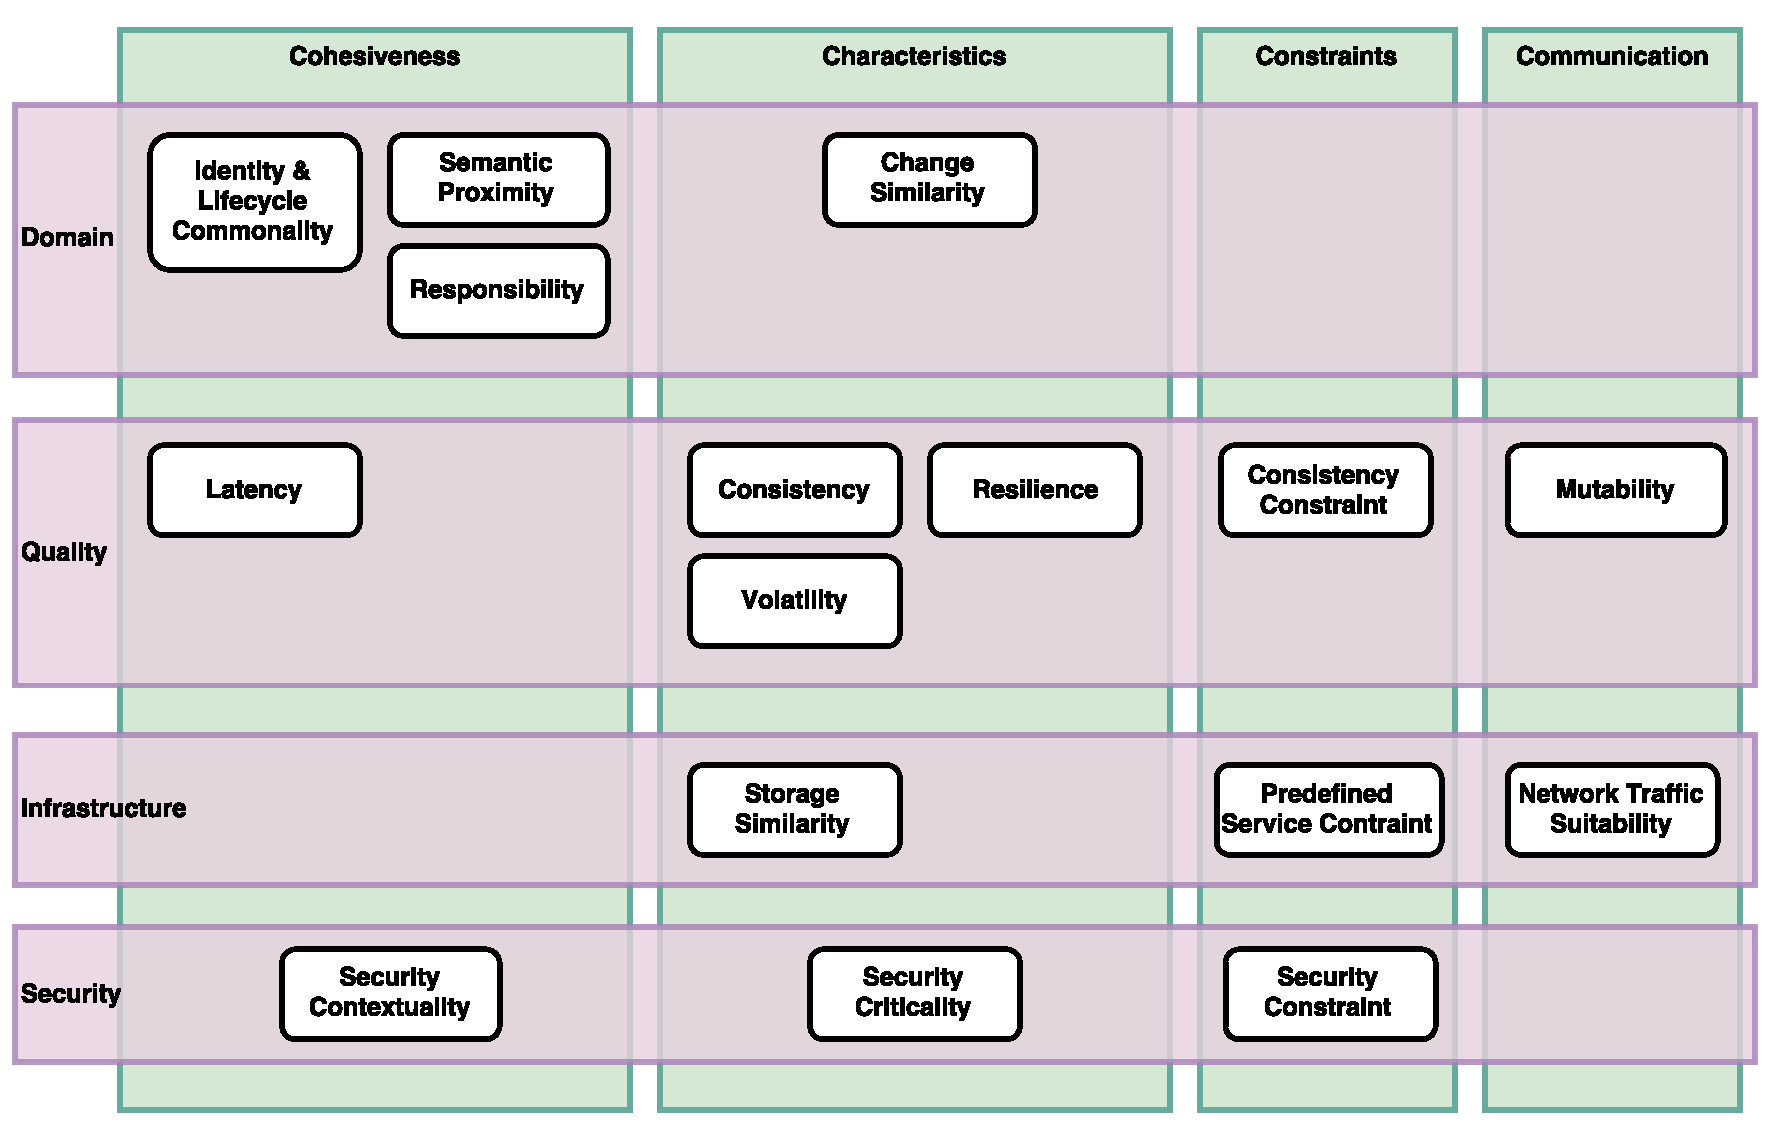
\includegraphics[scale=0.5]{diagrams/CouplingCatalog.pdf}
	\caption{Coupling criteria grid}
	\label{fig:cc_grid}
\end{figure}

The grid columns and rows represent the following partitions:

\begin{description}
	\item[Cohesiveness] - The fields should be in the same service.	\item[Characteristics] - The service should not contain different styles of a characteristic. A style is concrete value of a characteristic. E.g. \enquote{High}, \enquote{Eventually}, and \enquote{Weak} are styles of the characteristic \enquote{Consistency}.
	\item[Constraints] - The fields must be distributed amongst different services or the fields must form a service. (No fields are assigned to another service; no fields are added to this service.)
	\item[Domain] The fields originate from the context of a a specific business domain.
	\item[Quality] The fields involve quality attributes.
	\item[Infrastructure] The fields are resources and require specific hardware to be operated.
	\item[Security] The fields involve security requirements.

\end{description}

We specified all coupling criteria listed in the grid in the following \enquote{CC cards}. All cards share the following information:

\begin{description}
\item[Description] Explains the coupling criteria in more details.
\item[User Representation] Lists the familiar concepts that can be used to feed the coupling information into the Service Cutter.
\item[Literature] References the coupling criteria to descriptions in existing literature.
\item[Styles] Cards of type \enquote{characteristic} list different styles of a coupling criteria that should be separated.
\item[Type] Denominates the algorithm that is used for decomposition. %TODO add reference to implementation chapter
\end{description}

\newcommand{\ccCard}[7] {
\begin{minipage}{\linewidth}
	\begin{framed}
	\textbf{#1 #2}
	
		\begin{description}[leftmargin=!,labelwidth=\widthof{\bfseries User Representation}]
		\item[Description] #3
		\item[User Representation] #4 %TODO source?
		%\ifx #5\empty  #5 \fi
		\ifthenelse{\equal{#5}{}}{}{\item[Styles] #5}
		\item[Literature] #6
		\item[Type] #7
		\end{description}
	
	\end{framed}
\end{minipage}
}
\ccCard{CC-1}{Identity \& Lifecycle Commonality}{Data that belongs to the same identity and therefore shares a common lifecycle.}{UML class diagrams (Same Class, Composition, Inheritance)}{}{Evans?\cite{evans2003domain}.}{Cohesiveness}

\ccCard{CC-2}{Semantic Proximity}{Two fields are semantically when they have a natural connection. Semantic proximity originates from coherent field updates or aggregations in UML class diagram.}{Coherent field updates in Use Cases or User Stories. Aggregation or association relationships in UML class diagrams.}{}{Single Responsibility Priciple by Martin\cite{SRP}}{Cohesiveness}
%todo literature based on use case driven services?

\ccCard{CC-3}{Security Constraint}{Two fields are semantically related but must not reside in the same context. This restriction can be established by an external party such as a certification authority or an internal design team.}{A demilitarized zone, regulations, or certifications requiring separation of data.}{}{}{Constraint}

\ccCard{CC-4}{Security Criticality}{Criticality of a field in case of data loss or a privacy violation. Represents the reputational or financial risk when the data is disclosed unauthorized parties.}{}{High, Medium, Low}{}{Characteristic}

\ccCard{CC-5}{Resilience}{Data and their connected operations have varying availability constraints. Some parts are critical while others can be unavailable for some time.}{}{Critical, Normal, Low}{}{Characteristic}

\ccCard{CC-6}{Volatility}{Data can be classified by its update frequency or volatility. }{Use Cases may be equipped with a frequency that can be mapped the underlying data. Another approach is to use the data types Master Data (regularly), Reference Data (rarely), Transaction Data (often), and Inventory Data (often) to determine the volatility.}{Often, Regularly, Rarely}{}{Characteristic}
%TODO add literature (datentypen?)

\ccCard{CC-7}{Consistency}{Some data loses its value if not kept consistent together while other data is more tolerant to inconsistencies.}{}{High, Eventually, Weak}{}{Characteristic}

\ccCard{CC-8}{Storage Similarity}{Storage that is required to persist all instances of a data field.}{}{Small (KB), Medium (MB), Large (GB), Huge (TB)}{}{Characteristic}

\ccCard{CC-9}{Network Traffic Similarity}{Volume of data transferred on the network. This information is defined by how often an instance of a field is read or written, how many instances of the field exist and the size of the field.}{}{Low (1/d or small size), Medium (1/min or medium size), High (1/s or large size), Huge (100/s or huge size)}{}{Characteristic}

\ccCard{CC-10}{Change Similarity}{How often Change Requests are going to be implemented in this area.}{}{Often (every month), Rarely (every year), Never}{}{Characteristic}

\ccCard{CC-11}{Predefined Service Constraint}{There might be the following reasons why some parts forcefully needs to be modeled in the same service. Those may include technology optimizations, organizational reasons, or existing legacy services.}{}{}{}{Constraint}
%TODO quote conweys law here or in CC-13

\ccCard{CC-12}{Latency}{This group of fields share a common latency requirement and remote calls should be avoided. Therefore it is beneficial to model them in the same service.}{}{}{}{Cohesiveness}

\ccCard{CC-13}{Responsibility}{The same role or department is responsible for this group of fields. Mixing services with diverging responsibilities increases the maintenance complexity.}{}{}{}{Cohesiveness}

\ccCard{CC-14}{Security Contextuality}{The same role or department is allowed to see or process the fields. Mixing security contexts complicates authentication and authorization implementations.}{}{}{}{Cohesiveness}

% \ccCard{CC-}{}{}{}{}{}{}

%TODO mutability

\subsection{What is a good Decomposition Solution?}
\label{sec:decompositionRequirements}

Based on the Coupling Criteria described above, we define a good decomposition solution as following:

\begin{enumerate}
	\item Not violating any constraints.
	\item Putting as few data fields together which have different characteristics as possible.
	\item Each Service should depend on as few data of other Services as possible (A use case should cross as few Service boundaries as possible).
	\item The amount of data fields a Service depends on should be similar for all Services.
	%TODO: This is a cite by Udi Dahan internal workshop material, how can we cite this?
	\item Not too many Services which leads to the nanoservice antipattern\cite{nanoservice}.
	\item Not too few Services, which leads to a monolithic architecture.
\end{enumerate}

\section{Existing Decomposition Solutions}

TODO: Market analysis. Java Code analysis, GraphGist project to analyse service dependencies etc...




%TODO User stories as most important criteria: check Ivar Jacobson, oose, a use case driven approach

%TODO: Should we describe non relevant coupling criteria as well? (Hiding design decisions etc, see CC catalog doc)

%TODO: (Bring result \& discussion already here?)
